\section{Question 1}

The data are shown on \autoref{q1_two_observations}.

\begin{figure}[!ht]
  \centering
  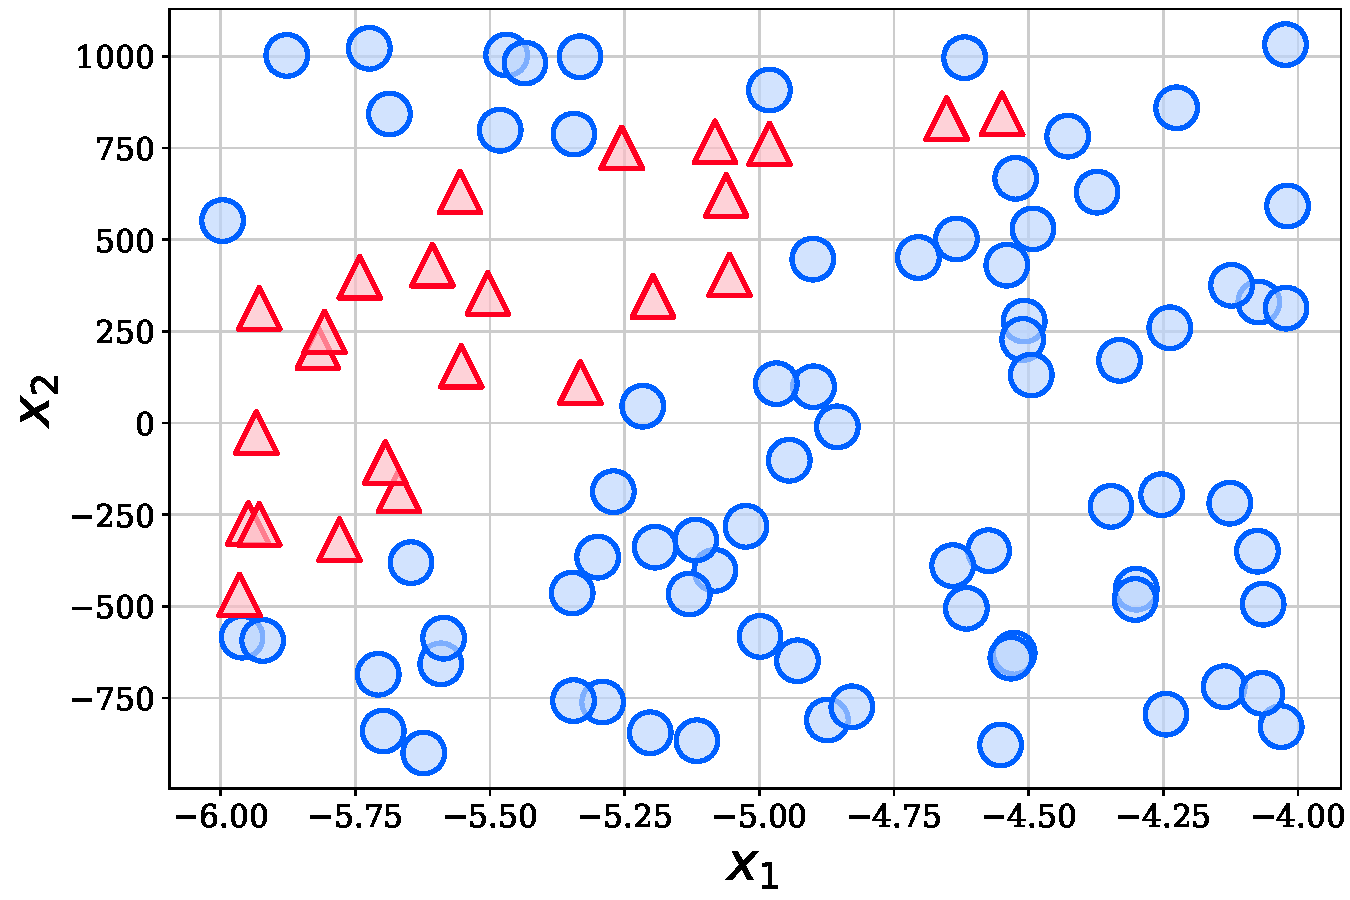
\includegraphics[width=1\textwidth]{figures/q1.pdf}
  \caption{Two types of observations. Code: q1.py.}
  \label{q1_two_observations}
\end{figure}

The diagram of the neural network is shown on \autoref{q1_network_diagram}. I choose the sigmoid activation function for the hidden layer nodes, because it's a common one. This is a classification task with just a single binary output (0 or 1). Therefore, for simplicity, I chose a single output node with no activation function (i.e. $f(x) = x$). If there were more than one output nodes than I could try a softmax function, but here it's not necessary.

\begin{figure}[!ht]
  \centering
  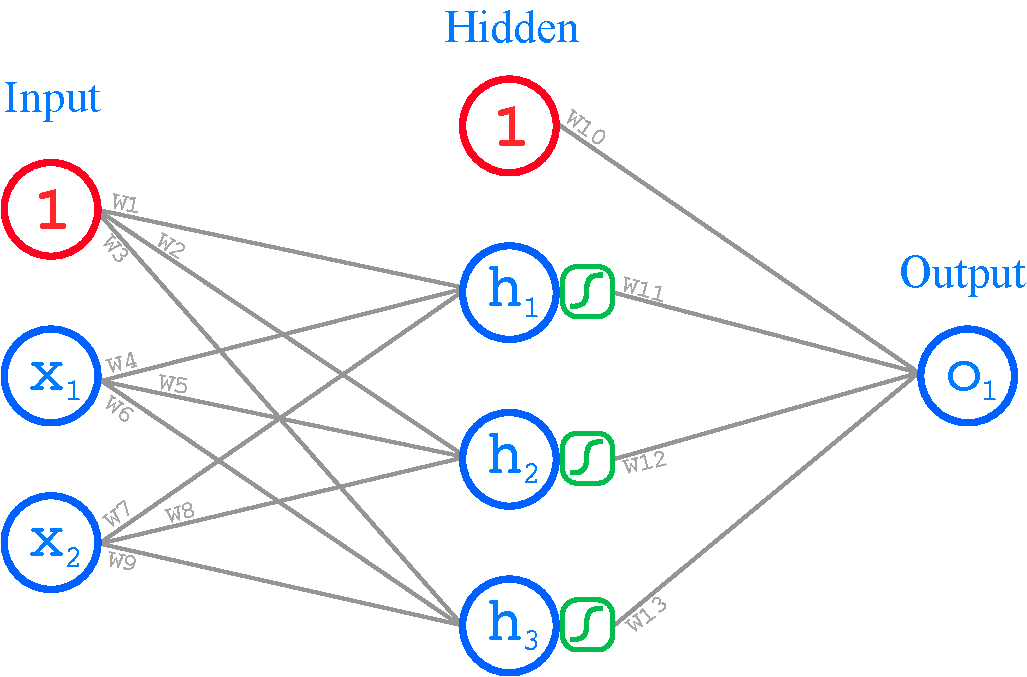
\includegraphics[width=0.7\textwidth]{figures/q1_neural_network.pdf}
  \caption{Diagram of the neural network containing two inputs, single hidden layer with three nodes and a single output layer.}
  \label{q1_network_diagram}
\end{figure}


\subsection{Removing sigmoid from output layer in Lecture 13 code example}

\begin{figure}[!ht]
  \centering
  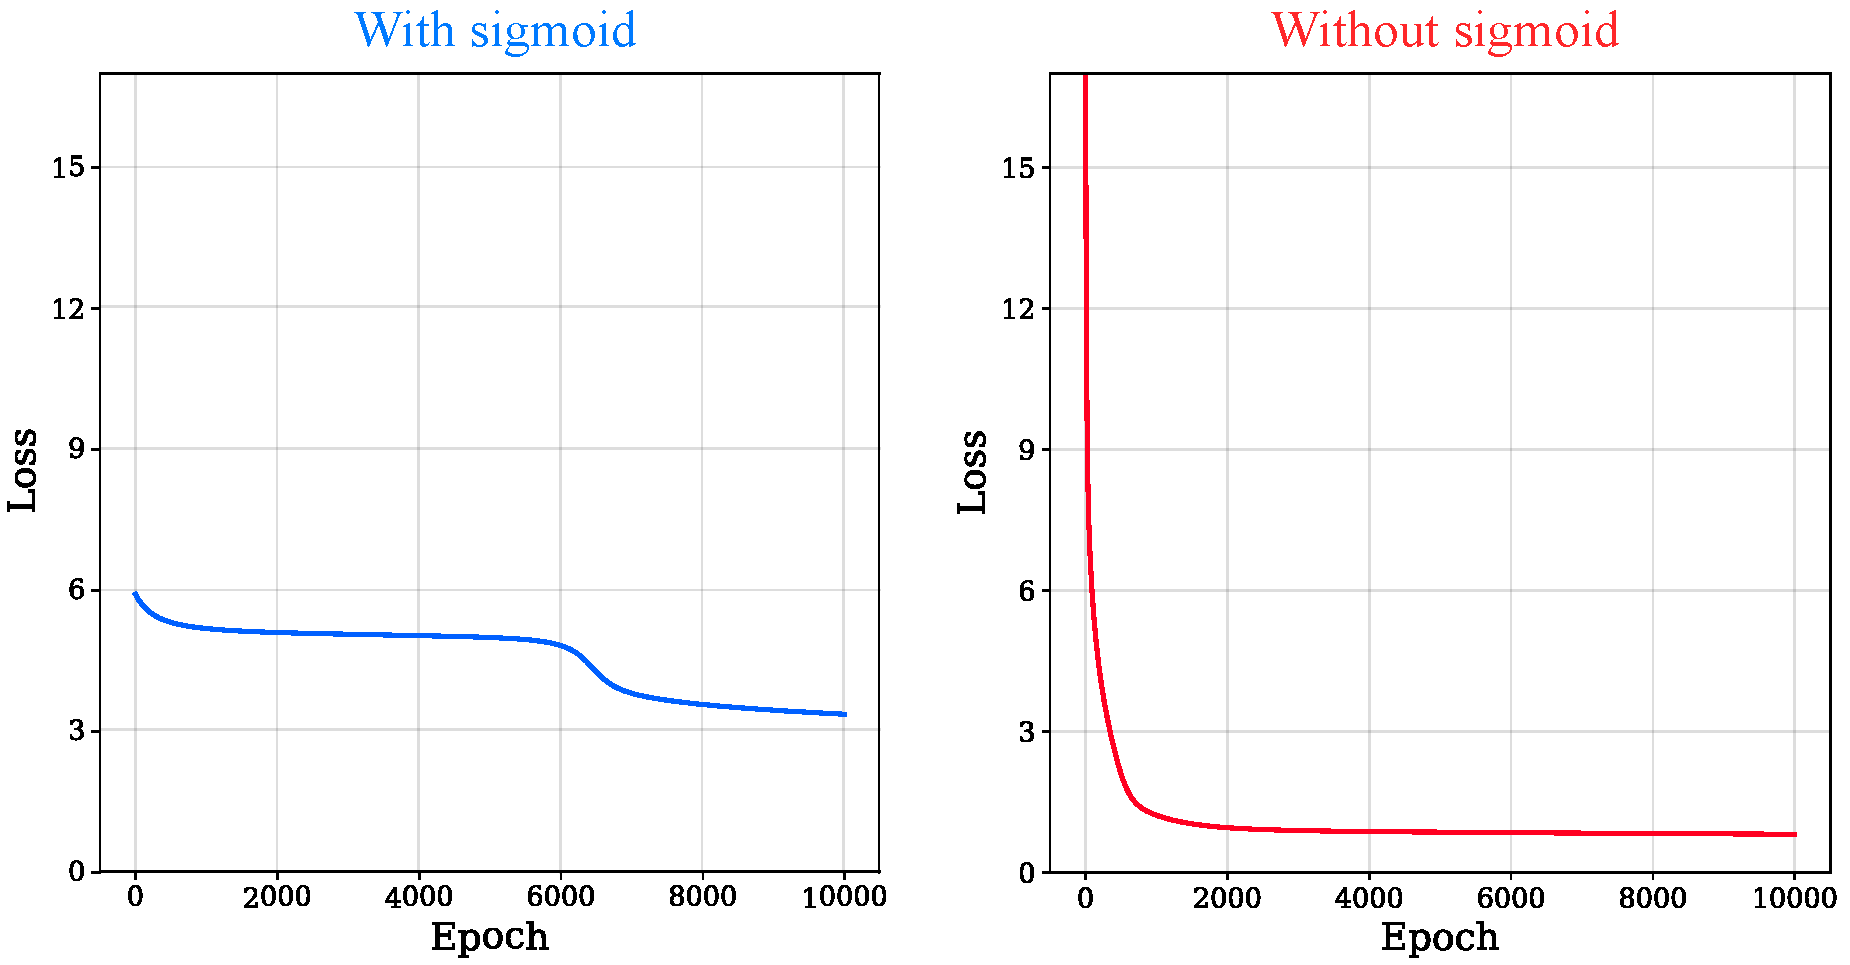
\includegraphics[width=0.7\textwidth]{figures/lecture13_loss_compared.pdf}
  \caption{Diagram of the neural network containing two inputs, single hidden layer with three nodes and a single output layer.}
  \label{q1_network_diagram}
\end{figure}



